\chapter{Document versions}

\vspace{0.5cm}
\begin{table}[H]
	\centering
	\begin{tabular}{|l|r|r|r|} \hline
	Version & Date & Comments & Responsible \\ \hline \hline
	1.0 & 12/11/2021 & First draft & Standard Committee \\ \hline
	2.0 & 2/12/2021 & Final document & Standard Committee \\ \hline
	2.1 & 28/12/2021 & Fixed typos, format change & Standard Committee \\ \hline
	\end{tabular}
	\caption{Document versions}
	\label{tab:label}
\end{table}


\chapter{Introduction and scope}

This document intends to define the specifications of a protocol for the transmission of 0.5KB of data, encoded in UNICODE, from a randomly selected transceiver to a receiver passing through different intermediate nodes within 5 minutes.

To achieve the objective, the protocol and the functionality for the application described above is defined through a flow diagram. Additionally, the structure and packets required for the transmission are detailed.

Note that the protocol described within this document is designed for having minimum three transceivers: one transmitter, one receiver and one intermediate node. In a generic way, the protocol will be defined taking into account that there will be $N$ nodes. The protocol described must be robust enough to send the file to all $N$ available nodes.

We assume that each device counts with at least one button for transmission start and one button for transmission stop, in addition to some mechanism for indicating that it’s the first of the chain. The first device will be in charge of reading the text file from the USB memory; this will indicate it’s the first device.






\chapter{Procedure specification}
The protocol is based on the Stop \& Wait mechanism, with a token-based multiple access control to avoid collision between packets on the air. The communication always links just two nodes at the same time and on the air there is just one packet being sent.

The main idea is to implement a simple protocol that enables the transfer of a file through all the nodes in the network in an easy and reliable manner. The Network OSI layer is based on packet transmission (TCP based) whose content is based in a mix between Stop \& Wait and Neighbour Discovery.

The reader can refer to \Cref{fig:m1-png} and \Cref{fig:m2-png} for a visual explanation of the packets to be sent and received.
\begin{figure}[H] \centering
	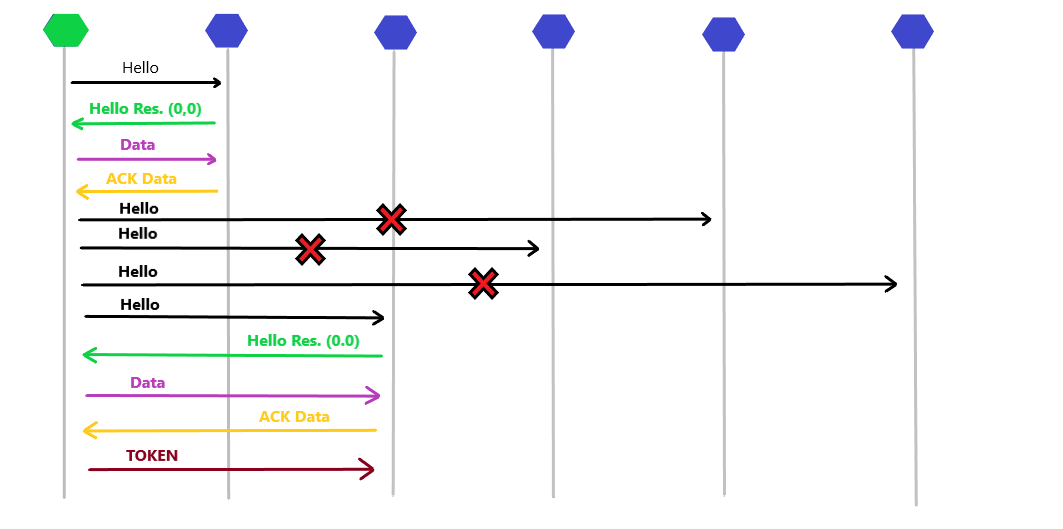
\includegraphics[width=1\textwidth]{m1.png}
	\caption{Flow diagram, 1}
	\label{fig:m1-png}
\end{figure}

\begin{figure}[H] \centering
	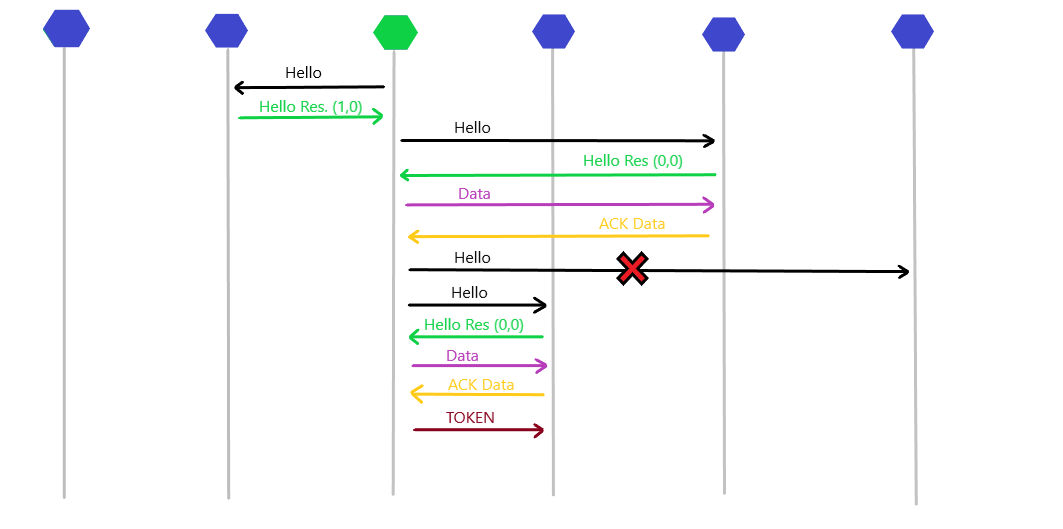
\includegraphics[width=1\textwidth]{m2.png}
	\caption{Flow diagram, 2}
	\label{fig:m2-png}
\end{figure}


The protocol uses a token that indicates who is the user able to transmit, only the user holding the token, let it be called \textit{token user} for the purpose of this document, can transmit at that time. Any other user is only allowed to answer to the token user with a \textit{HELLO RESPONSE} or an \textit{ACK}, either a \textit{DATA ACK} or a \textit{TOKEN ACK} depending on the circumstances. Aside from handling who is able to transmit at all times, the token also has the purpose to keep track of how many users have the file at the moment. To pass the token to another user, the message \textit{TOKEN} is used.

One of the protocol objectives is to send the file to as many users as possible, so the user holding the token will try to contact all the other users in the network using a \textit{HELLO} message. For every user who answers with a \textit{HELLO RESPONSE} message indicating that it does not have the file, the token user will send the file to them.

To send the messages, the token user will follow an order to avoid collisions. It will start by sending the \textit{HELLO} message to one user, wait for an answer and then two situations might happen; it answers that it does not have the file, or it answers that it already has got the file from a previous transmission or does not answer. If it does not answer or answers it already has the file, the token user will try to contact the next user and send a \textit{HELLO} message to him. If it answers that it does not have the file it will send it to him and once finished send \textit{HELLO} to the next user. This process is repeated until the token user has tried to establish contact with all the users in the network, one by one. Finally, the token user will send the token to the last user with whom it has successfully established contact and sent the file. The token will indicate to the other user that it can transmit. Together with the token a message containing the IDs of the nodes who have already had the data will be sent.


The communication to send the file starts when the token user receives a \textit{HELLO RESPONSE} indicating that the user does not have the file. Then the user will start transmitting the file in different \textit{DATA} packets, waiting for an \textit{ACK} response for every packet, before sending the next one. If the packet fails, i.e., either the transmitter receives a negative response or it doesn’t receive any after an established timeout, the packet is sent again. The last packet will be indicated with the \textit{End of Transmission} bit.

When a user receives the token and it indicates that all the expected users (or users in the network) already have the file, it will stop trying to transmit any packet and the process will finish. Otherwise, it can happen that some users for some reason have not been able to establish a connection properly with their neighbours and have skipped the transmission process. In this case, a user will receive the token indicating that a number of users different from the expected in the network have the file. When that happens the process will start again and the token will try to contact all users again. However, it might happen that the node is too far away from the missing users and does not receive any answer from them. Then the user will send the token to any user who answers and has not had the token yet, so they can try to reach them. On the other hand, it might happen that all the answers indicate that they already have the file and already have had the token. In this situation the system will pass the token randomly to a user, so it tries again to reach the missing users. This situation will be repeated until it finally contacts the missing users and the transmission succeeds or it is ended by the five minutes timeout.




The reader can check \Cref{chapter:errors} to gain insight on the delays and retries imposed.


\Cref{fig:flowchart-pdf} depicts a state machine for one node.
\begin{figure}[H] \centering
	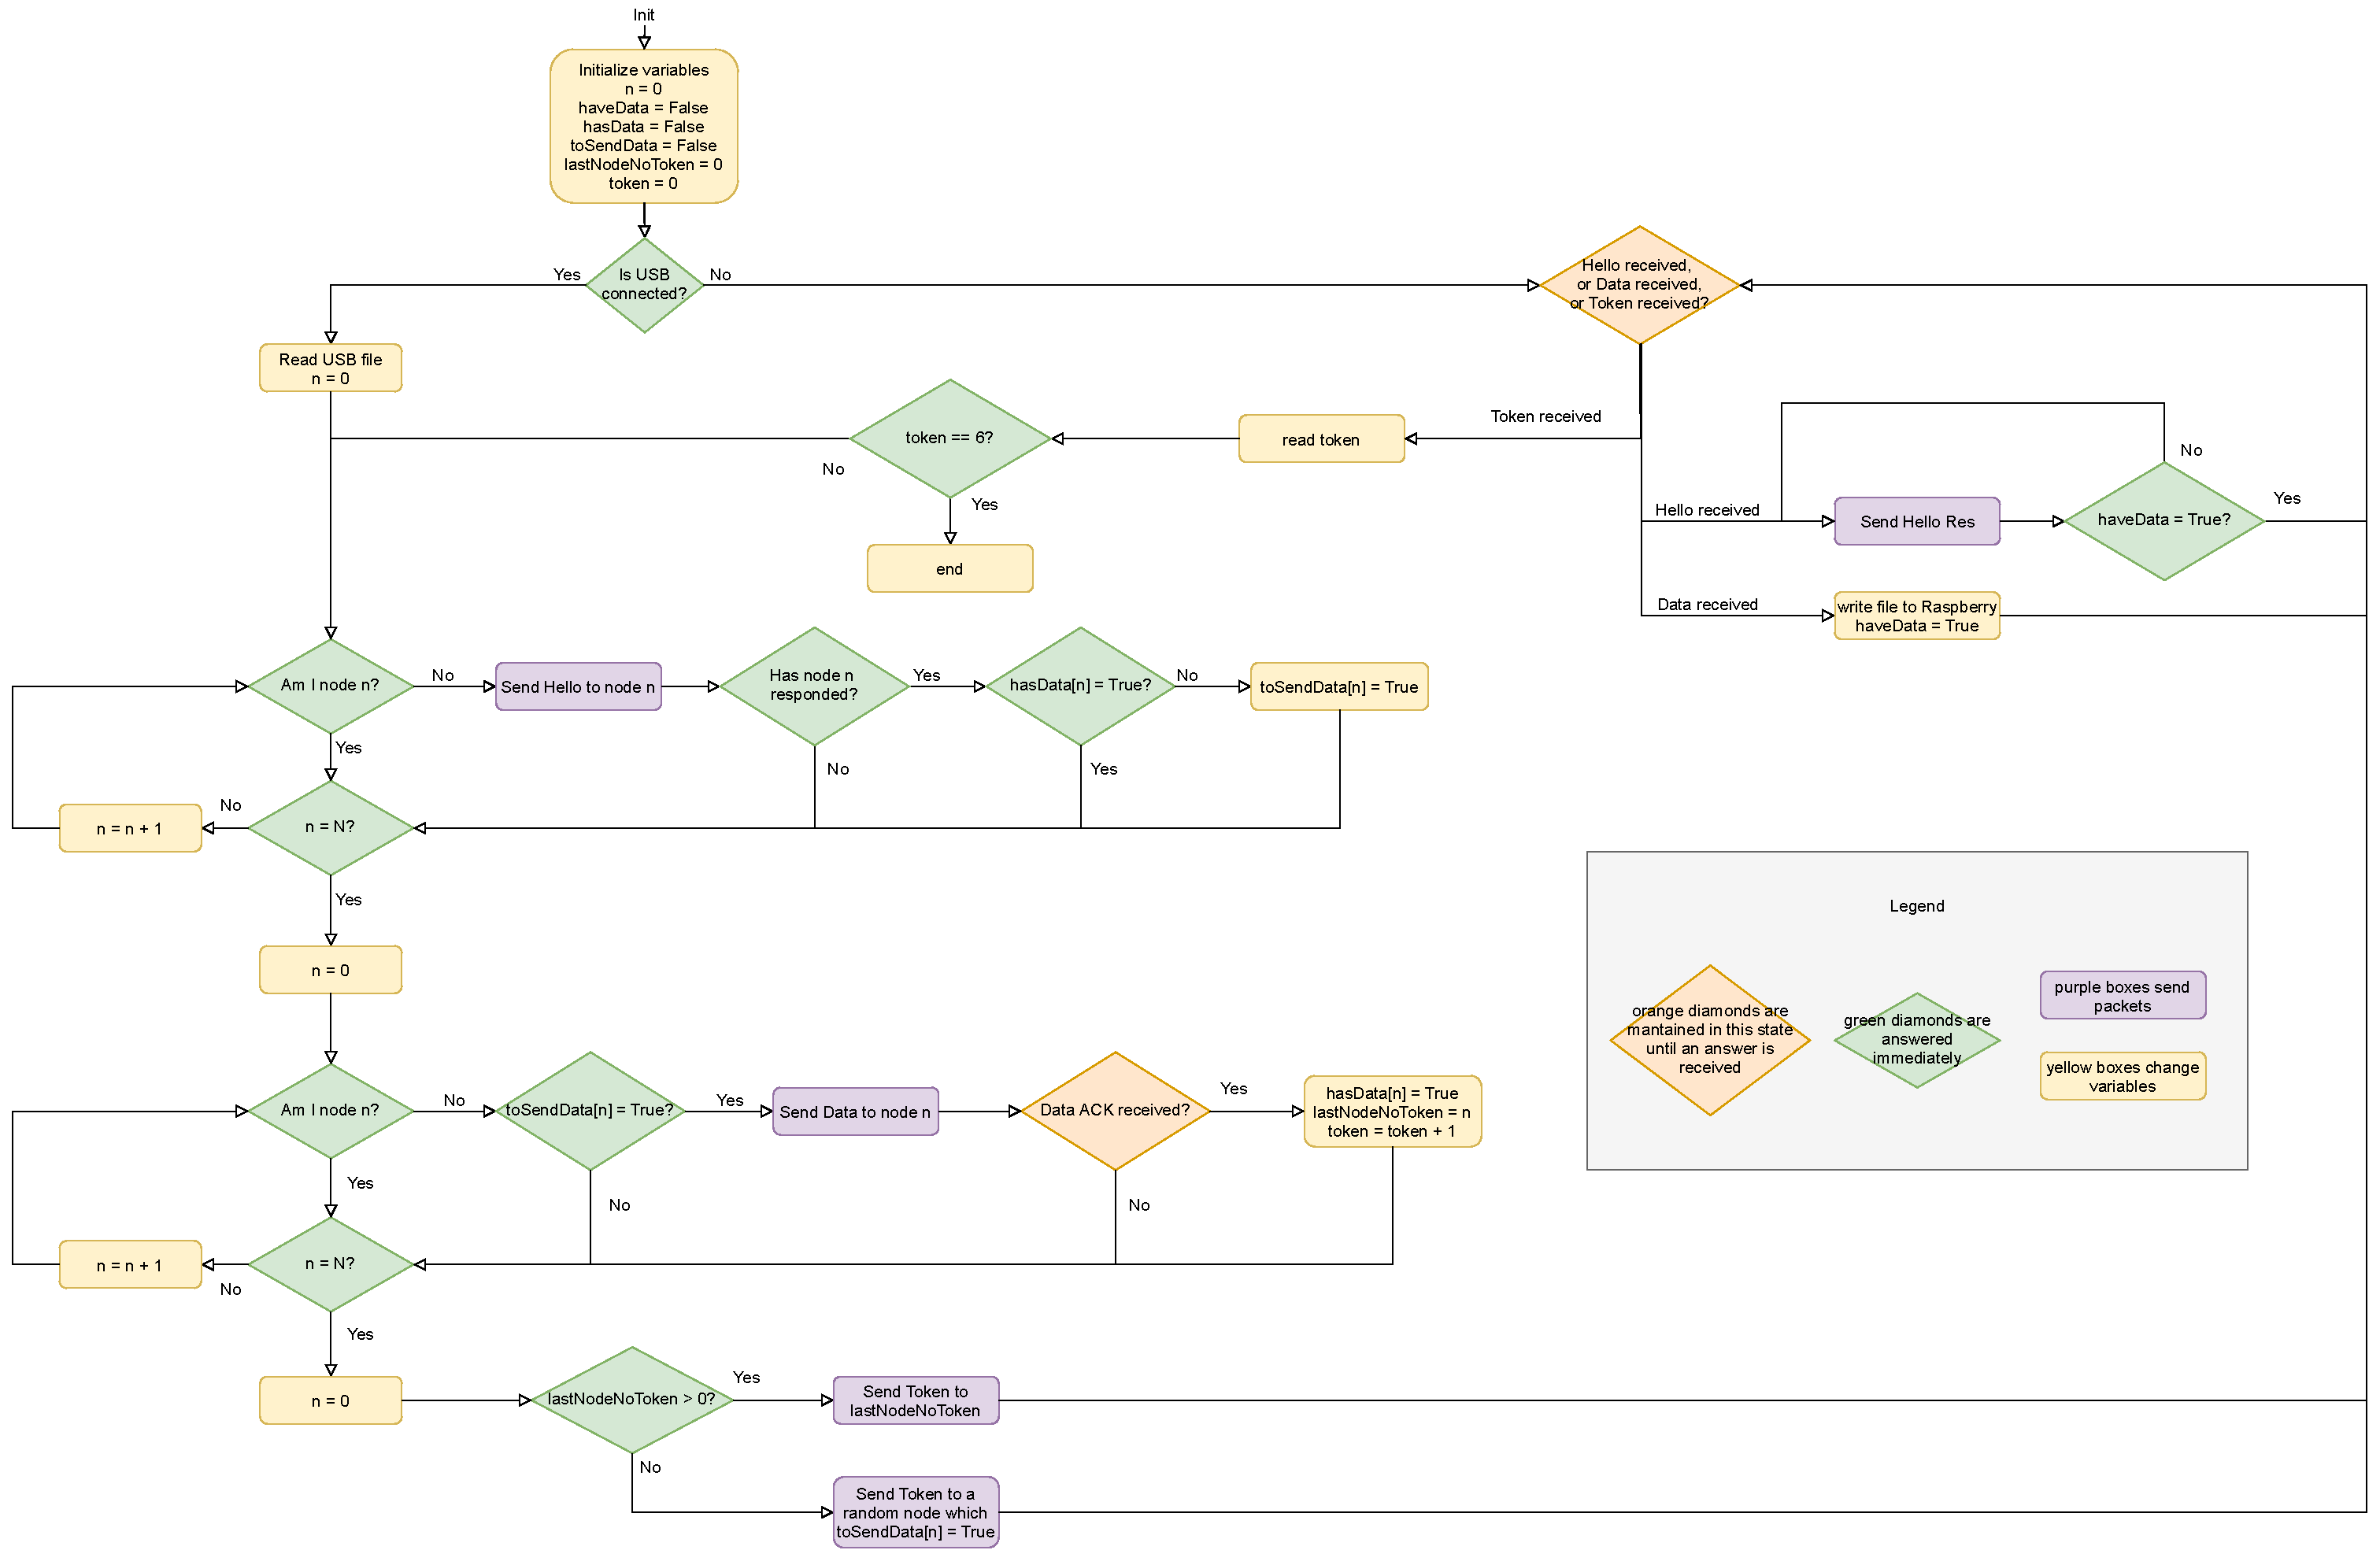
\includegraphics[width=1\textwidth]{flowchart.pdf}
	\caption{Flowchart}
	\label{fig:flowchart-pdf}
\end{figure}

\Cref{fig:flowchart-pdf-2} shows the same figure in a landscape page, to appreciate better the text and details.
\clearpage
\thispagestyle{empty}
\newgeometry{left=0.1cm, right=0.1cm, top=3cm, bottom=0.1cm}%Change margins
\begin{landscape}

\begin{figure}[H] \centering
	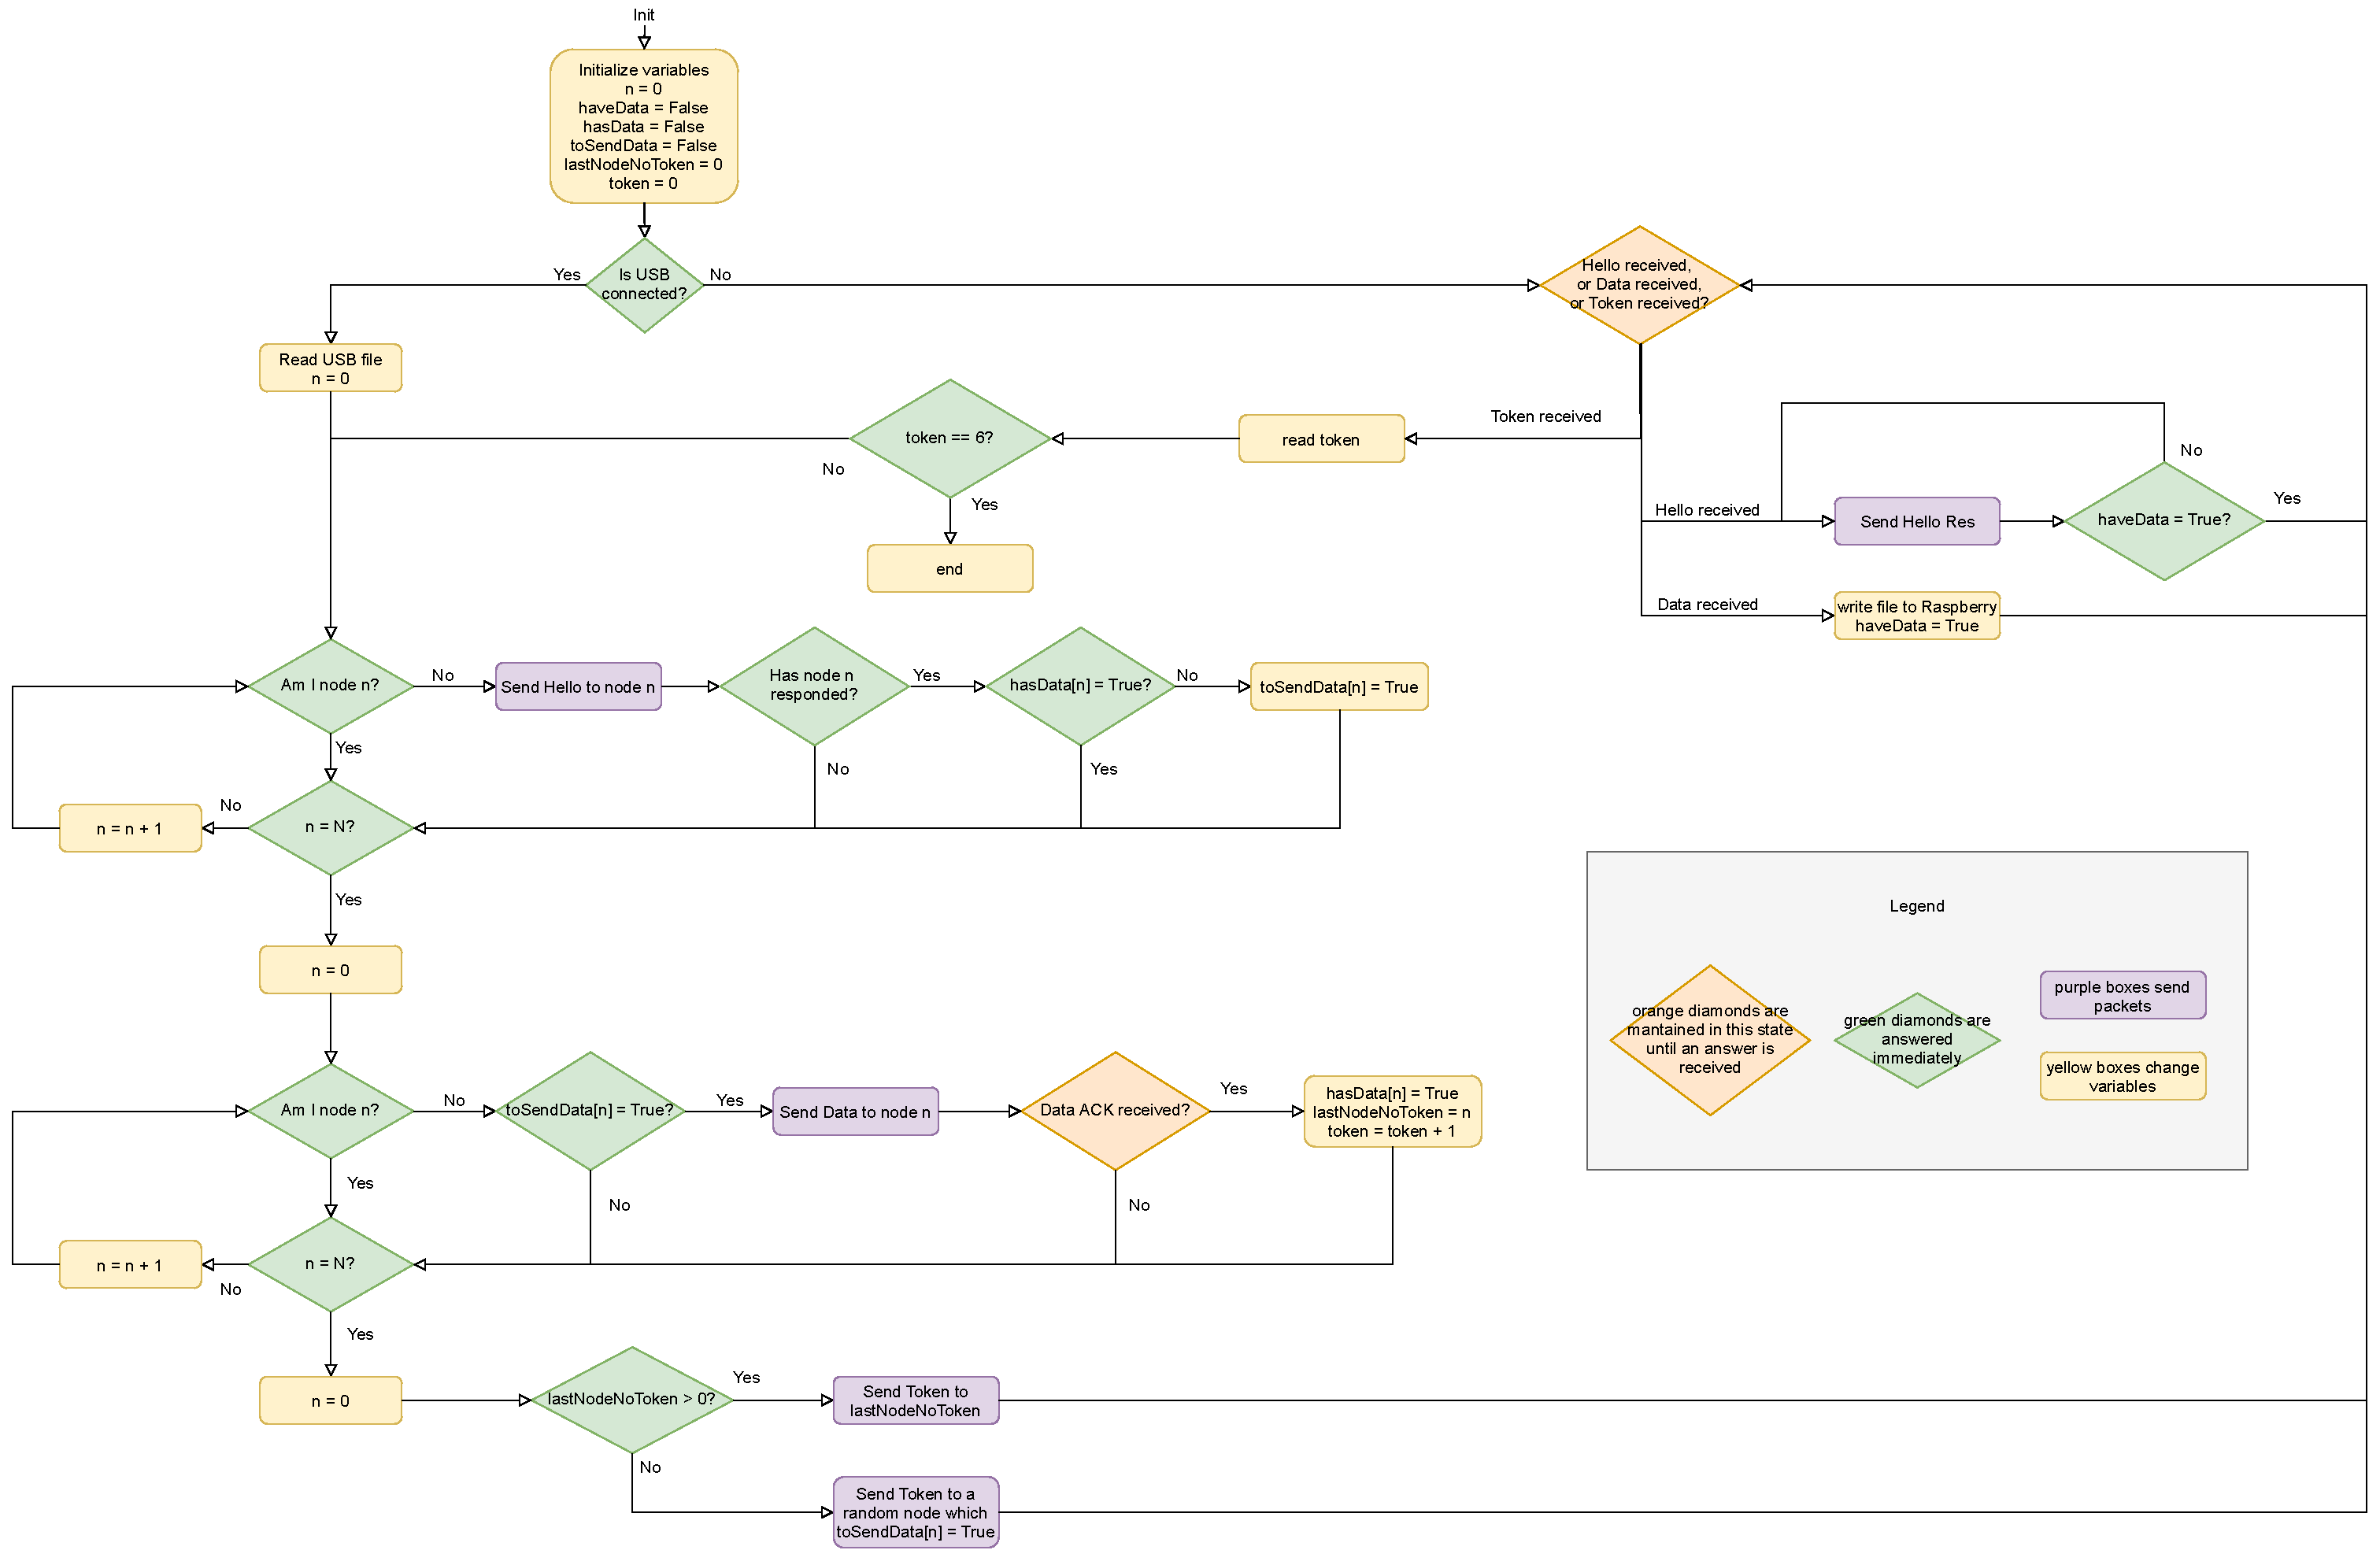
\includegraphics[width=1.42\textwidth]{flowchart.pdf}
	\caption{Flowchart, landscape view}
	\label{fig:flowchart-pdf-2}
\end{figure}

\end{landscape}

\restoregeometry



\chapter{Packet structure}
The following defines the different packages used and their structure. Note that the packets marked with an S are the packets sent by the node that has the token and the ones marked with R are the ones sent by the nodes that do not have the token in response to each of the S packets.
\begin{itemize}
	\item (S) \textit{HELLO}: Packet sent by the node that has the token to discover the nodes next to it.
	\item (R) \textit{HELLO RESPONSE}: A packet sent by a node that has received a \textit{HELLO} packet, to indicate to its transmitter that it is within range. With this package the node will also inform if it has had the token, and if it has the data.
	\item (S) \textit{DATA}: Packet sent by the node that has the token containing a part of the text file to be sent. Multiple data packets will transmit the total file.
	\item (R) \textit{DATA ACK}: Packet sent by the node that has received a \textit{DATA} packet to inform that it has correctly (or incorrectly) received the packet.
	\item (S) \textit{TOKEN}: Packet sent by the node that has the token to pass the token to another node.
	\item (R) \textit{TOKEN ACK}: Packet sent by the node that has received a \textit{TOKEN} packet to inform that it has correctly (or incorrectly) received the \texit{TOKEN}.
\end{itemize}

Each of the previously introduced packet types has a fixed part, same for all types, and a variable part, which depends on each type. Note: to simplify the protocol, packets will always be $32$ bytes long, so the packet definitions below will fill the first bytes required, and the rest will be padded with zeros.

\begin{figure}[H] \centering
	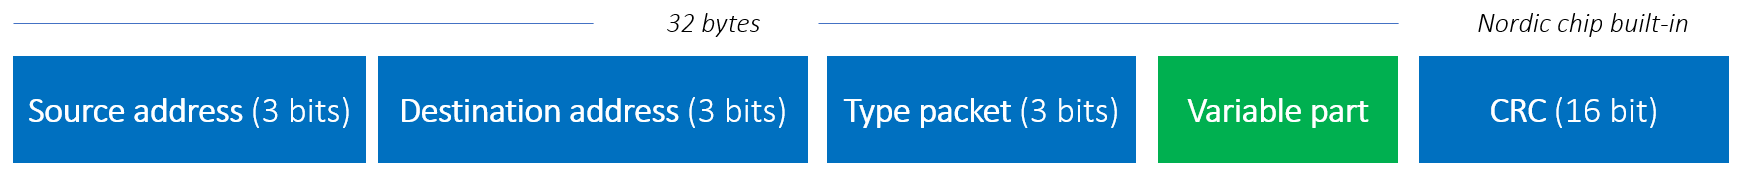
\includegraphics[width=0.8\textwidth]{1.png}
	\caption{Complete packet structure}
	\label{fig:1-png}
\end{figure}

The \texit{Source address} and \textit{Destination address}, as we have 6 nodes, will range from $0$ to $5$. Each node on the network will have a fixed address within this 0-5 range. Each of the packet’s types defined before has the following code (which is identified in the type packet field), shown in \Cref{tab:label}.
\begin{table}[H]
	\centering
	\begin{tabular}{|l|r|} \hline
		Packet type & Code \\ \hline \hline	
		\textit{HELLO} & 000 \\ \hline
		\textit{HELLO RESPONSE} & 001 \\ \hline
		\textit{DATA} & 010 \\ \hline
		\textit{DATA ACK} & 011 \\ \hline
		\textit{TOKEN} & 100 \\ \hline
		\textit{TOKEN ACK} & 101 \\ \hline
	\end{tabular}
	\caption{Packet type codes}
	\label{tab:label}
\end{table}

The variable part for each packet type is defined below.


\section{HELLO}
No variable part.


\section{HELLO RESPONSE}
The \textit{have data} field indicates if the node has the data (1) or not (0). The \textit{had token} field indicates if the node has had the token (1) or not (0).

\begin{figure}[H] \centering
	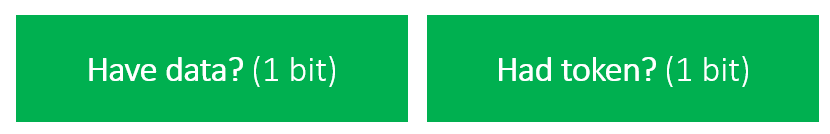
\includegraphics[width=0.4\textwidth]{2.png}
	\caption{\textit{HELLO RESPONSE} packet variable part}
	\label{fig:2-png}
\end{figure}

\section{DATA}
The \textit{length} field indicates how many bytes is the payload actually. This is useful for the last packet, that can have a different length than the rest of the packets. The \textit{End Of Transmission} (EoT) field, if 1 indicates the last packet. The \textit{SN (Sequence Number)} allows identificate the origin of the transmission packet. Finally, the \textit{payload} contains the actual text file data.

\begin{figure}[H] \centering
	
\includegraphics[width=0.8\textwidth]{3.png}
	\caption{\texit{DATA} packet variable part}
	\label{fig:3-png}
\end{figure}

\section{DATA ACK}
The \textit{SeqNum (Sequence Number)} identifies the packet that we are acknowledging for the stop & wait protocol. And \textit{ACK} (1) indicates the packet has been received correctly, and \textit{NACK} (0) the contrary, and is required a retransmission.

\begin{figure}[H] \centering
	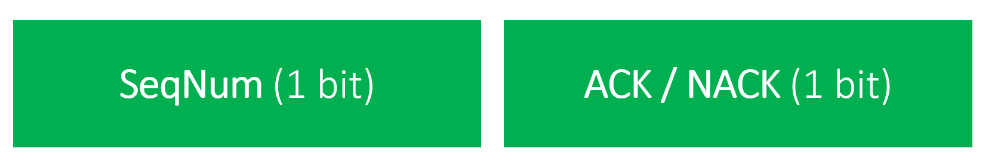
\includegraphics[width=0.4\textwidth]{4.png}
	\caption{\texit{DATA ACK} packet variable part}
	\label{fig:4-png}
\end{figure}


\section{TOKEN}
The \textit{Num. Recv. Data} indicates the nodes that have received the data. If a node receives a token with this field at 6, it can stop the transmission as all the nodes have the data.

\begin{figure}[H] \centering
	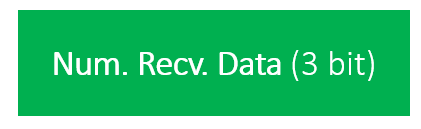
\includegraphics[width=0.2\textwidth]{5.png}
	\caption{\textit{TOKEN} packet variable part}
	\label{fig:5-png}
\end{figure}

\section{TOKEN ACK}
And \textit{ACK (1)} indicates the packet has been received correctly, and \textit{NACK (0)} the contrary, and is required a retransmission.

\begin{figure}[H] \centering
	
\includegraphics[width=0.2\textwidth]{6.png}
	\caption{\textit{TOKEN ACK} packet variable part}
	\label{fig:6-png}
\end{figure}










